\begin{savequote}[75mm]
You are like my father in some ways.\\
WHAT RESEMBLANCE DO YOU SEE\\
You are not very aggressive but I think you don't want me to notice that.\\
WHAT MAKES YOU THINK I AM NOT VERY AGGRESSIVE
\qauthor{A conversation with ELIZA (from Weizenbaum 1966)}
\end{savequote}
\chapter{Question Generation and Response}

\section{Introduction}

In this chapter, I describe how the Luna Rating System fits within the broader context of existing AI research. A test that requires excessive additional work beyond the immediate products of research would not be effective in recruiting participants, and would therefore fail as a practical driver of research. Fortunately, LRS invites direct applications of two subfields of Natural Language Processing: Question Generation (QG) and Question Answering (QA). The Interview Phase of the Luna Game, in which players must compose original questions and reason about expected answers, is a straightforward application of QG. The Response Phase, which requires each player to answer the questions of the other player, similarly corresponds to QA. The Guess Phase does not have an obvious corollary problem in existing research, but its structure suggests an intriguing new problem, which I characterize in Chapter 5.

As a test for AI, LRS only requires a solution to QA. The presupposition of the test is that responses are sufficient to encapsulate intelligence. Researchers who wish to use LRS purely as a test may therefore choose to avoid the challenges of QG by defining a simple interviewing scheme, such as selection from a fixed set of questions. However, a researcher whose focus is QG may utilize Luna to gather human responses to the questions generated by a new algorithm. Moreover, for researchers who wish to take a more holistic approach to AI, the Luna Game offers intriguing applications of both QG and QA. Thus I offer a review of work on both fields as part of this introduction of the Luna Rating System.

\section{Interview Phase: an Application of Question Generation}

\subsection{Scope of Question Generation}

Question Generation, as the name suggests, is the study of automatically generating linguistically valid questions. In practice, the generated questions must pertain to a given topic, which is often defined implicitly by providing a collection of natural language samples as input to the generator. A slightly stronger requirement, sometimes included to narrow the scope of the task, is that the generated questions must be directly answered within the provided text \cite{rus2011question, heilman2011automatic} . These text samples may be relatively short, like a single sentence \cite{ali2010automatic, rus2011question}, or longer, like a paragraph \cite{mannem2010question} or a full natural language corpus {heilman2011automatic}. They may be factual, like the encyclopedia examples, or fictional, like a short story derived from a simulated world. Practical applications of QG often rely on a standardized format for text inputs. 

The reliance on text input in existing studies of QG may be seen as both beneficial and detrimental in the context of the Luna Game. For one, questions derived from text often have clear correct answers, which simplifies the task of assessing responses. On the other hand, there are many probing questions that could not be reasonably constructed on the basis of text. (For example, there are uncountably many arithmetic problems that have never been asked!) In this sense, the practical scope of QG forms a subset of the general problem suggested by the Interview Phase, but the ultimate aims of both are concordant. 

The success of questions generated for the purpose of the Interview Phase may be measured according to the precision and accuracy with which the author may subsequently guess the respondent's Smarts Rating. In existing research on QG, the metric used to assess the quality of generated questions is varied. A straightforward approach used in recent work is to count the number of unique questions generated from the input text. This metric avoids the difficulty of defining question quality but subsequently provides no guarantees about the question's content. An alternative method relies on manual human input to determine the quality of each question. While potentially more meaningful, this metric can be costly, subjective, and vulnerable to human error. The challenge of defining a metric that is both semantically meaningful and efficiently evaluated is arguably the greatest barrier between QG and mainstream NLP research.

\subsection{Previous Work on Question Generation}

Question Generation is often motivated by the prospect of automated intelligent educational tools \cite{graesser2005scaffolding, heilman2011automatic}. A system capable of generating a set of reasonable questions from an academic text would be invaluable for learning and assessment, especially in the era of MOOCs and other online educational resources. Heilman's work, which I describe in more detail below, is primarily motivated by this educational potential \cite{heilman2011automatic}. In the specific context of English language learning, Kunichika et al. (2004) create an interactive system that generates questions from a novice textbook and then adaptively presents a series of questions to students based on their previous responses \cite{kunichika2004automated}. Xu et al. (2010) provide a similar game-based system for learning Mandarin \cite{xu2009automatic}. Other motivations for QG include assisting human questioning, participating in general dialogue \cite{walker2001spot}, and providing synthetic datasets for the related task of Question Answering (see Chapter 5). Piwek et al. (2008) make a broad case for QG as a task of interest for AI and Computational Linguistics, advocating an ``open-minded approach... [towards] a new and hopefully soon burgeoning area of research" \cite{piwek2008generating}.

If surface-level questions suffice for an application, and questions need not be diverse in style, there are several simple QG options available. One coarse approach is the Cloze procedure, in which words from the input text are randomly replaced with blanks for the responder to complete \cite{taylor1953cloze}. For example, the input text ``George Washington was born in Virginia'' might generate the question ``George Washington was born in $\rule{2cm}{0.05mm}$''. The next level of sophistication involves applying templates to text in search of specific syntax patterns, and then applying one of several predefined transformations accordingly. For example, the previous input text might be matched and transformed to the question ``Where was George Washington born?'' or ``Who was born in Virginia?'' \cite{gates2008automatically, kunichika2004automated, heilman2011automatic}. A variant of this template-based strategy is employed by ELIZA, the therapist-like chatterbot developed in 1966 by Weizenbaum \cite{weizenbaum1966eliza}. Template-based methods may also be used to generate multiple choice questions \cite{mitkov2006computer}. Work by Ali et al. (2010) relies on sentence classification and syntax parsing before applying transformations to generate questions \cite{ali2010automatic}.  Wang et al. (2007) use a similar transformation-based procedure in the domain of medical texts \cite{wang2007automatic}. While template methods produce syntactically correct questions that are more appropriate for applications like dialogue, it is not clear that they produce deeper semantics than the simpler Cloze procedure. 

In 2010, a Question Generation Shared Task and Evaluation Challenge (QGSTEC) was announced, leading to an uptick of interest on the problem and a set of more sophisticated methods \cite{rus2011question}. QGSTEC included two tasks: QG from sentences, and QG from paragraphs. In both cases, the questions generated by the five contestants were evaluated manually on the basis of relevance, question type, correctness, ambiguity, and variety. This human-dependent evaluation unfortunately restricts the long term impact of QGSTEC, since new methods cannot be reliably compared with the baselines set in the contest. Nonetheless, the challenge succeeded in bolstering work on QGSTEC. Ali et al. entered a straightforward syntax-based method using Part of Speech tagging and Named Entity analysis \cite{ali2010automatic}. Pal et al. took a similar approach with an additional focus on clausal boundaries \cite{pal2010qgstec}. Yao \& Zhang broached semantics directly by converting inputs into Minimal Recursion Semantics representations and then applying transformations into questions \cite{yao2010question}. Varga \& Ha modified an existing multiple choice question generator to fit the specification of the task \cite{vargaha}. Mannem et al., the only team to attempt the paragraph to question subtask, used predicate argument structures to generate many more questions than required, and then ranked the candidate questions to select the final output \cite{mannem2010question}. 

The \textit{overgenerating transformations and ranking} of Mannem et al. has been championed by Heilman, who completed his dissertation on the subject in 2011 \cite{heilman2010extracting, heilman2010good, heilman2011automatic}. The paradigm is a promising approach to QG, since it separates the task of generating all syntactically possible questions from the task of selecting semantically valid and useful questions. In Heilman's work, the overgeneration step is accomplished through syntax pattern matching and manually encoded transformation rule applications. Ranking is then performed using a variety natural language features. The ranking step is shown to double the acceptability of generated questions, as defined by human judges. The dataset tested is larger than that of QGSTEC, but still strictly limited by the dependency on human input.

\subsection{Question Generation: Future Directions}

Overgenerating transformations and ranking is a promising approach to QG, but previous efforts have been severely limited by the requirement of manual human question labeling to train the ranking function. The standard procedure has been to overgenerate transformations, solicit humans to label the results as valid or invalid, and then train a ranking function that is optimized to award high rankings to valid questions. The theory is that this ranking function can subsequently be applied to other datasets of unlabeled questions generated via transformations or other procedures. Ranking according to statistical analyses of standard natural language features has been shown to double the percentage of valid questions present in the top 20\% ranked generated questions. While this result demonstrates the potential of ranking, it leaves significant room for improvement, as 50-60\% of invalid questions remain in the output \cite{heilman2011automatic}. 

Ranking functions would presumably benefit from vastly more data to train on, but such human-labelled datasets remain scarce. Meanwhile, large unlabeled datasets of questions generated by humans are abundant. Future research on QG may be able to utilize these unlabeled datasets by converting them into datasets of real coherent questions and fake incoherent questions created from noisily swapping out words in the real questions. A binary classifier could then be trained on this augmented dataset, learning to distinguish valid question from invalid ones. This trained classifier could then be used in place of the ranking function to identify valid questions from overgenerated sets. This paradigm of using the distributional hypothesis to recasting problems as binary classification has been successfully applied in recent work \cite{collobert2011natural}, but has not yet been considered in QG. This approach could make advances in deep learning available to QG for the first time. 

\section{Response Phase: an Application of Question Answering}

\subsection{Scope of Question Answering}

The Response Phase of the Luna Game bears immediate resemblance to a subfield of Natural Language Processing known as Question Answering (Q\&A). Q\&A is defined as the general problem of automatically responding to any question posed in natural language \cite{andrenucci2005automated, hirschman2001natural}. The breadth of the problem can be a blessing and a curse. Such a broad definition effectively encompasses all of artificial intelligence; it is argued that the problem can only be solved by a machine with true general AI \cite{yampolskiy2013turing}. This completeness is what makes Q\&A an appropriate centerpiece in a test for AI. At the same time, the tremendous scope of the problem can be a barrier to progress. The lack of common structure between possible questions gives researchers little to exploit. Moreover, the task of assessing a candidate solution to Q\&A presents several challenges and ambiguities. How should test questions be selected from the extraordinarily large number of possible question topics and forms? How should answers be assessed, especially in the case that a question may be subjective, or have several equally valid answers? These difficult questions have discouraged research on the general Q\&A problem in favor of more narrow tasks.

In pursuit of tractability, researchers have explored a variety of restrictions on Q\&A. These restrictions may apply to question content, question format, or answer format. Question content may be limited by focusing on a fixed source of information that assumedly contains all answers. The size and structure of this source can greatly influence the difficulty of the task. In one extreme, the source might be all of Wikipedia in natural language form, with no further direction nor additional parsing provided. An easier source would be a structured knowledge base like Freebase, which organizes relational information in a very precise and predictable way \cite{bollacker2008freebase}. The source may also be small and question-specific, e.g. a reading comprehension task that supplies text samples and asks the reader to infer answers based only on the samples \cite{richardson2013mctest}. With a source established, question formats are often limited so that there is a clear single correct answer. For example, the questions may be true or false, multiple choice, or single word answers. The answers themselves may be further limited to natural language fragments, or even single words, that are lifted directly from the provided text. Each of these potential restrictions on Q\&A represents a tradeoff between tractability and generalizability. As the field progresses, the range of what is tractable has expanded, allowing for commensurate improvements on more general problems.

\subsection{Previous Work on Question Answering}

The motivation for Question Answering is abundant and self-evident. Every problem in AI --- in all fields, in fact --- can be phrased as a question. Imagine a machine that could answer every possible question. It could be asked, for example, ``What are the answers to all possible questions, ordered by importance to humanity?'' Of course, practical research on Q\&A is driven by much more immediate ambitions. Q\&A is often presented within the context of the World Wide Web and restricted to factual questions \cite{cucerzan2005factoid, ravichandran2002learning, kwok2001scaling}. A web-based system capable of directly answering user queries would be the prize possession of a search engine company. Indeed, with the introduction of Knowledge Panels with search responses that are derived from the Knowledge Graph, Google is increasingly blurring the lines between Information Retrieval and Q\&A \cite{singhal2012introducing}. Another extrinsic, if toy motivation for Q\&A is the television trivia game Jeopardy!, which inspired IBM's DeepQA team to develop Watson, perhaps the most famous Q\&A system to date \cite{ferrucci2012introduction}. Additionally, personal assistant technologies, like the DARPA PAL project (which later became Apple's Siri) and the Amazon Echo, all rely on Q\&A for their core functionality \cite{aron2011innovative, tsiao2007natural}. The corporate origin of each of these examples is representative; there is enormous product-driven demand for progress on Q\&A.

Q\&A has been studied consistently for over half a century. The majority of work on the subject falls into one of three categories: factoid Q\&A from structured knowledge bases, factoid Q\&A from free text, and non-factoid Q\&A. Given a structured knowledge base, i.e. a list of logical predicates, Q\&A essentially reduces to the subproblem of mapping natural language to queries, either explicitly or with the addition of a latent term \cite{yao2014information, zelle1996learning}. With multiple possible answers, an additional selection step is required, which usually involves a ranking function similar to those used for Question Generation. Factoid Q\&A from free text cannot take advantage of structured relations, and thus has the additional burden of parsing text from a natural language corpus in search of relevant information \cite{ravichandran2002learning}. While this added challenge is considerable, these algorithms typically also have access to significantly more data than their knowledge base oriented counterparts \cite{brill2001data, hermann2015teaching}. This setup makes the factoid Q\&A from free text especially appropriate for deep learning techniques. Both types of factoid Q\&A leave open the possibility of training an algorithm on an external dataset of facts before the questions are asked. In contrast, non-factoid Q\&A forces an algorithm to discover answers to questions on an ad-hoc basis \cite{soricut2004automatic}. Non-factoid Q\&A typically includes a fictional story as part of the prompt, and then ask a question which has an answer that can only be inferred from the story. While the information retrieval portion of the task is somewhat simplified, the challenges of automatic reasoning and inference are brought to the fore.

Another distinguishing feature among approaches to Q\&A is the extent to which questions and answers are parsed into intermediate representations. Recent efforts have attempted to learn mappings directly from questions to answers without forming any representations in between. Before the rise of deep learning, such efforts would have been unthinkable due to the incredibly large space of possible questions and answers in any practical domain \cite{hirschman2001natural}. For example, Figure \ref{fig:NLPQA}, reproduced from \cite{androutsopoulos1995natural}, provides an example of how an end-to-end system for Q\&A was divided into modules in 1995. The system includes modules for syntax parsing, semantic rule application, database querying, and output generation, each which must be separately addressed. A 2001 review by Burger et al. divides Q\&A even further into 12 subproblems, including Question Classes, Question Processing, Context, Data Sources, Answer Extraction, and Answer Formulation among others \cite{burger2001issues}. The current state of the art suggests that this level of granularity does not necessarily lead to better performance.  

\begin{figure}[h]
\centerline{%
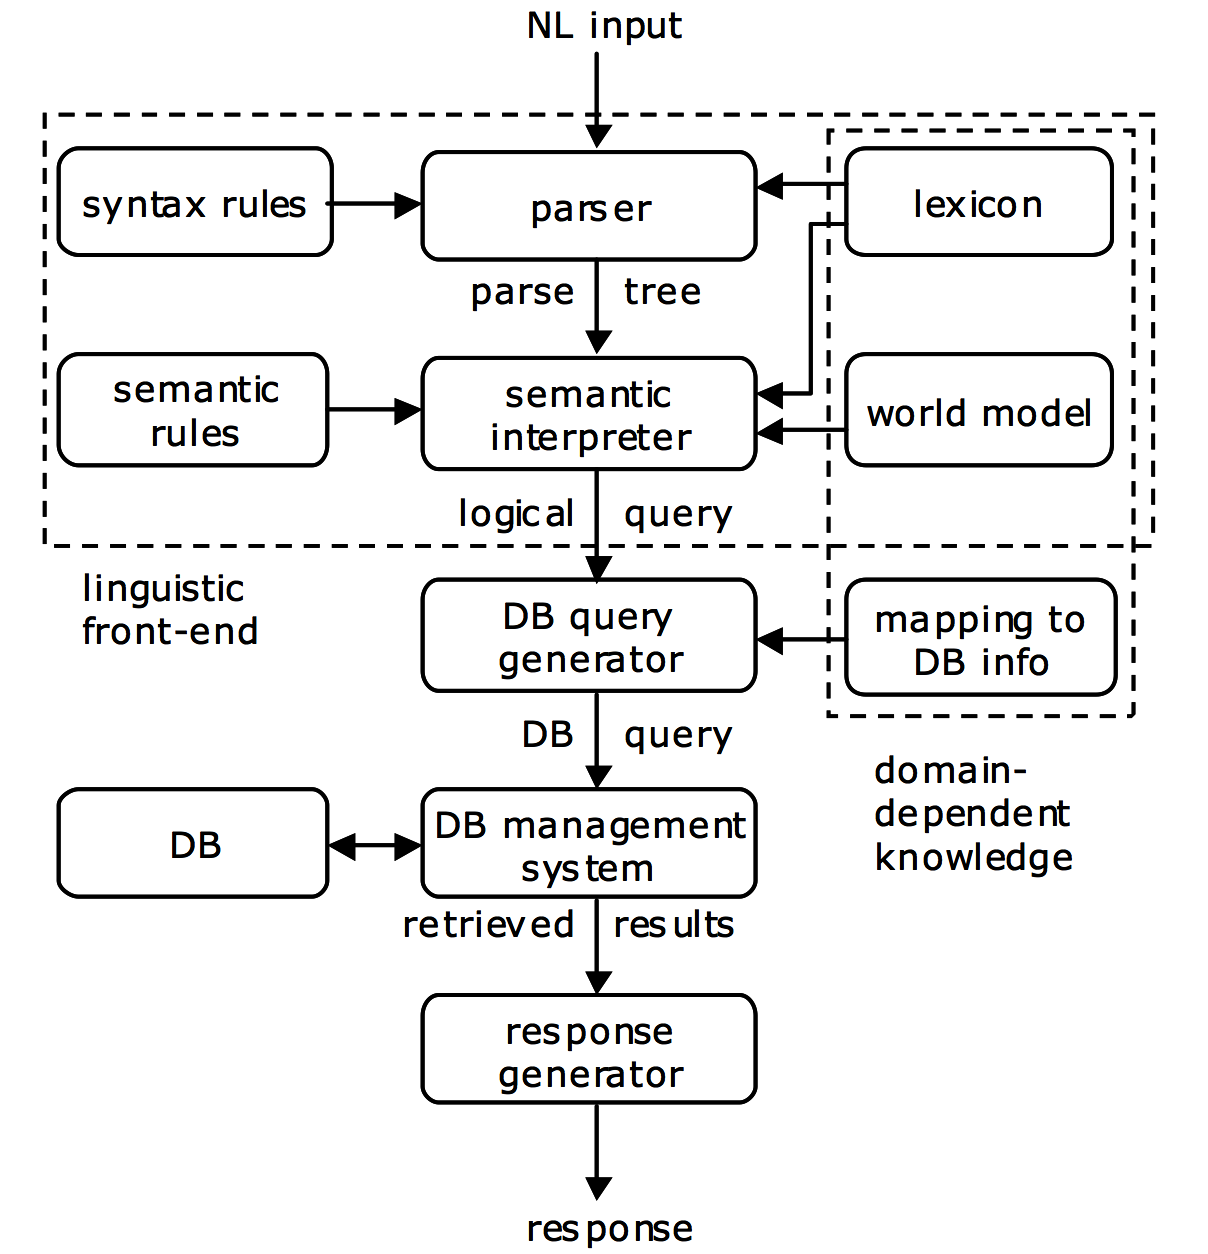
\includegraphics[width=0.5\textwidth]{figures/NLPQA.png}}%
\caption{Architecture of a typical Natural Language system for Question Answering, from \cite{androutsopoulos1995natural}. The structure could be used in full or in part as a template for approaching the Response Problem.}
\label{fig:NLPQA}
\end{figure}

In 1999, a Q\&A task was added to the Text Retrieval Conference (TREC), an ongoing series of workshops in information retrieval that provides centralized benchmarks for many similar problems \cite{voorhees1999trec}. The dataset used for the task consists of 200 factoid short-answer questions, such as ``How many calories are there in a Big Mac?'', and provides a natural language corpus of newspaper articles and similar archives that somewhere contain the answers. The answers provided by the algorithms are assessed by human judges for validity, representing the same bottleneck of the Question Generation task discussed above. Nonetheless, the Q\&A TREC task, which was repeated every year from 1999 to 2007, enjoyed far more attention than the analogous QG task has thus far\cite{dang2007overview}. The datasets from the task have also been utilized consistently in subsequent work and have been used as a benchmark to establish progress. Indeed, the concentration of 21st century Q\&A research around the factoid free text subproblem is likely due in part to the prominence of the TREC task \cite{hirschman2001natural}.

Recent work by Facebook AI could potentially serve as an epicenter for research on the non-factoid subproblem. In a paper titled \textit{Towards AI Complete Question Answering: A Set of Prerequisite Toy Tasks}, Weston et al. define 20 simplified non-factoid question answering subtasks, forming the bAbI task \cite{weston2015towards}. The subtasks are designed to strip away many of the superfluous complexities of naturally occurring text, instead focusing on core concepts one-by-one. Following the non-factoid question paradigm discussed above, questions are presented with a collection of statements containing the desired answer. For example, the simplest type of question is the Single Supporting Fact, in which the answer may be derived directly from a single provided statement. All questions in bAbI are based on a simulated world involving several agents and objects with various possible actions. In relying on a simple simulation, as did Winograd in earlier work \cite{winograd1971procedures}, bAbI is able to provide an ideal amount of unpredictability while still keeping the task focused on specific types of questions. The bAbI task has already inspired advances in deep learning approaches to Q\&A, including the notable introduction of Memory Networks \cite{sukhbaatar2015weakly}.

\subsection{Question Answering: The Way Forward}

As evidenced by its inclusion in TREC, Q\&A has long been viewed as an extension of information retrieval \cite{kolomiyets2011survey}. Classical information retrieval returns a document containing relevant information in response to a query. Q\&A accepts the same type of query and returns a passage or parsed passage of relevant text from a similar source. The introduction of bAbI, with its non-factoid questions based on a simple simulated world, signifies a shift in the conception of Q\&A. Research on the problem is now reaching towards sophisticated reasoning in small worlds, as opposed to simple reasoning in large worlds. This shift is a critical step in the pursuit of AI-complete Q\&A. Simple factoid questions represent a very limited subset of the questions that a true AI will be expected to answer. As progress on the existing bAbI tasks continue, it will be expedient to gradually add more sophisticated tasks to continue to guide research.

Work on bAbI has already produced algorithms that are able to handle an impressive range of question types pertaining to the small simulated world. Information retrieval efforts continue in parallel, making it possible to answer simple questions over increasingly large sets of semantics. A critical question for the future of Q\&A is how to close the gap between these two problems. One approach would be to gradually scale solutions to bAbI tasks to larger worlds. A mirrored method would be to increase the level of sophistication in the questions that information retrieval algorithms are able to answer. A third, and potentially most promising strategy, would be to explicitly bridge the divide while maintaining the distinction between the two problems. In this scenario, a machine could learn relations between a very limited number of entities, in the spirit of bAbI. It could then learn about a vast number of entities without learning new relations using traditional information retrieval. Finally, a mapping between the entities in the bAbI task and the retrieved entities could be learned, and new relations between these retrieved entities could be inferred. 
%
%
%ROADMAP
%
%Nonetheless, researchers of the Response Problem can take inspiration and guidance from the substantial work done on Q\&A. Perhaps most enlightening is the manner in which Q\&A is decomposed into subproblems. The 2003 review by Burger et al. defines a roadmap for Q\&A that has often been followed by subsequent research \cite{burger03, kolomiyets11}. The subtasks include\footnote{There are twelve subtasks defined in \cite{burger03}, but the most notable are the first six, as the remaining six --- Real-Time Q\&A, Multilingual Q\&A, Interactive Q\&A, Advanced Q\&A, User Profiling, and Collaborative Q\&A --- go beyond the basic objective of Q\&A.} Question Classes, Question Processing, Context, Data Sources, Answer Extraction, and Answer Formulation. These six subtasks are sufficiently general that they may transfer to the Response Problem. Written two years later, the review by Andrenucci \& Sneiders distinguishes three main approaches to Q\&A: a Natural Language approach, an Information Retrieval approach, and a question template approach \cite{andrenucci05}. The three differ mainly in emphasis; the Natural Language approach focuses on the semantics of the question and answer, the Information Retrieval approach is chiefly concerned with the representation and access of information, and the question template approach deals almost exclusively with pattern matching questions and annotated information. Each of these approaches could in theory be generalized for the Response Problem, but the Natural Language approach, with its emphasis on semantics, is likely most appropriate. 
%
%Figure \ref{fig:NLPQA}, reproduced from \cite{androutsopoulos95}, provides an example of how an end-to-end system for Q\&A can be separated into modules. The first section of the system is dedicated to linguistic processing. At the lowest level, syntax rules and a lexicon are used to parse the natural language input a standard format that a semantic interpreter can process. Semantic rules, such as first-order logic, and a world model, which encodes relationships and constraints for elements of the semantic domain, are integrated to produce a logical query into a database. After the database processes the query, a final module converts the database output into a human-readable response. This architecture offers an example of how a system for the Response Problem could be structured. The syntax rules and lexicon may be already be ready for more general use. With a sufficiently advanced collection of semantic rules, world model, and database, the system could perform quite well. Of course, the level of advancement in each of these areas required for the Response Problem seems far beyond the reach of current AI.
%
%A system for Q\&A offers a solution to the Trivia-type questions in the Response Problem. Several other possible question types have their own corresponding areas of research. Commonsense reasoning \cite{davis15}, creativity \cite{oliveira15}, spatial reasoning \cite{freska15}, vision \cite{zheng15}, and emotional intelligence \cite{tawatsuji15} have all been formalized and are actively studied\footnote{In fact, each of the preceding citations came from 2015!} as subproblems in AI. Questions of opinion, and other questions that rely on a human identity, may be addressed with research in Dialogue, e.g. through a chatbot \cite{weizenbaum66}. One possible approach to the Response Problem is to detect the type of a question and then parcel it out to the appropriate sub solution. This method is in line with the ``bottom-up'' approach to AI. The analogous method, the development of one general mechanism for answering all questions in the Response Problem, aligns with the ``top-down'' approach. To gain insight into the current state of AI, each paradigm should be used for the Response Problem; the highest Smarts Rating of a single mechanism machine and the highest Smarts Rating of a machine that uses a combination of subproblems will both serve as illuminating indicators of progress.
%
%\subsection{Applications of Question Answering to Luna Games}

